\newpage
\chapter{Obtaining the weights}
\mbox{}\vspace{-\baselineskip}
\label{sect:weights}

The weight for each event is determined by exactly the same procedure that is described in Sect.~4 of the report~\cite{twopeg}. The weight factor is calculated according to Eq.~(4.7) from that section with the following three modifications.


%determined according the Eq.~(4.7) of the report~\cite{twopeg}, where 


%to the procedure described in Sect.~(4) of the report~\cite{twopeg} 


\begin{itemize}
\item Instead of the generated value $W_{sm}$, which is assumed to be smeared, the true value $W_{true}$ defined by Eq.~\eqref{w_fermi_nonsm} should be used for picking up the cross section. 

\item To combine the structure functions into the full virtual photoproduction cross section, one should use the values of  $\varepsilon_{T}$ and $\varepsilon_{L}$ calculated in the quasi-Lab frame according to Eqs.~\eqref{eps_t} and~\eqref{eps_l}. See the discussion in Sect.~\ref{sect:ambig}.
\item To obtain the electroproduction cross section from the virtual photoproduction one (mode $F_{flux}=1$), the virtual photon flux $\Gamma_{v}$ should also be calculated in the quasi-Lab system using the effective beam energy $\widetilde{E}_{beam}^{qL}$ introduced by Eqs.~\eqref{eq:in_part_qlab} and the value of $\varepsilon_{T}$ calculated according to Eq.~\eqref{eps_t} in the quasi-Lab frame.
\end{itemize}






Event distributions that illustrate this procedure are shown in Fig.~\ref{fig:weights_w_dep}. The plot (a) shows the comparison of two weighted event distributions, i.e. the $W$ distribution produced by TWOPEG for the case of free proton (green curve) is compared with the $W_{sm}$ distribution produced by TWOPEG-D (blue curve). The blue curve demonstrates the expected blurring of the resonance structure caused by Fermi smearing. The plot (b) compares the same green curve from free proton TWOPEG with the $W_{true}$ distribution produced by TWOPEG-D (purple curve) and reveals their intrinsic consistency. 

Figure~\ref{fig:weights_w_dep} (b) requires further clarifications. As it is written in Sect.~\ref{sect:gen_var}, TWOPEG-D flatly generates $W_{sm}$, while $W_{true}$ is calculated according to Eq.~\eqref{w_fermi_nonsm} and therefore loses the flatness of generation, being affected by the generation of the Fermi momentum. This is illustrated in Fig.~\ref{fig:weights_w_dep} (c), 
which shows the unweighted TWOPEG-D  distributions of $W_{sm}$ generated in a range 1.3~GeV $< W_{sm} <$ 1.9~GeV (blue curve) and the corresponding $W_{true}$ (purple curve).
While the former distribution is flat, the latter is not: it drops abruptly at the edges and has a plateau in the middle. This behavior is quite justified, since each value of $W_{true}$ can correspond to the sequence of  $W_{sm}$ symmetrically scattered into a certain range (see Fig.~\ref{fig:w_smear}). The Fermi momentum distribution forces most of the $W_{sm}$ values to be located in the vicinity of $W_{true}$ with a deviation of $50$-$100$~MeV, while wider deviations are significantly less probable. Hence, the plateau values of the  $W_{true}$ distribution manage to collect the majority of the corresponded $W_{sm}$ values within whole generated range, while the edge values of $W_{true}$  fail to achieve it. To saturate the edge regions of the $W_{true}$ distribution, the values of $W_{sm}$ should be generated in a wider range, as it is demonstrated in Fig.~\ref{fig:weights_w_dep} (d). To produce this plot, $W_{sm}$ was generated in a range 1.25~GeV $< W_{sm} <$ 2~GeV that leads to the almost full saturation of the $W_{true}$ distribution in a range 1.3~GeV $< W_{true} <$ 1.9~GeV. The comparison of the weighted distributions shown in Fig.~\ref{fig:weights_w_dep} (b) is plotted for the case of saturated unweighted $W_{true}$ distribution shown in Fig.~\ref{fig:weights_w_dep} (d).


\begin{figure}[!ht]
\begin{center}
\framebox{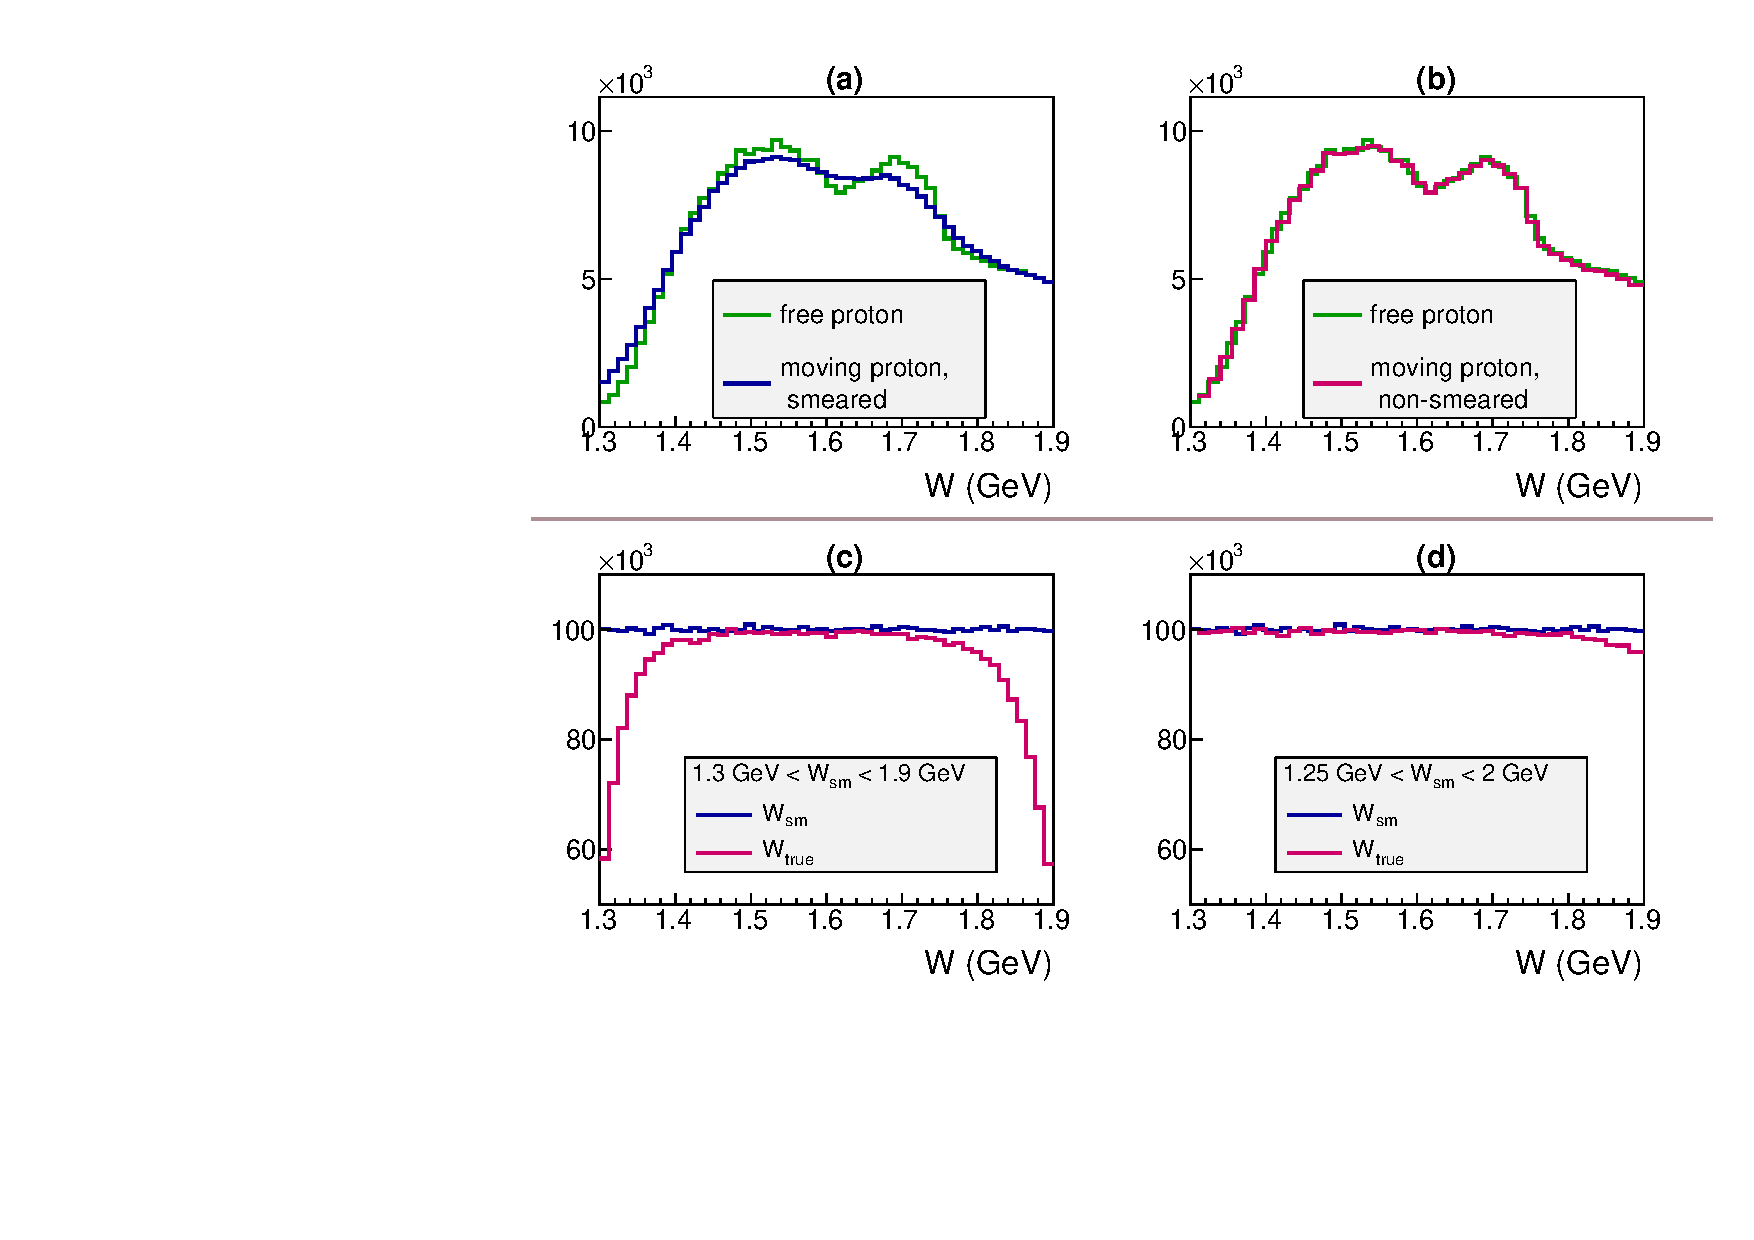
\includegraphics[width=16cm]{pictures/weights_w_dep2.pdf}}
\end{center}
\caption{\small {\bf(a)} The comparison of two weighted event distributions, i.e. the $W$ distribution produced by TWOPEG for the case of free proton (green curve) is compared with the $W_{sm}$ distribution produced by TWOPEG-D (blue curve). \\\textbf{(b)} The comparison of two weighted event distributions, i.e. the $W$ distribution produced by TWOPEG for the case of free proton (green curve) is compared with the $W_{true}$ distribution produced by TWOPEG-D (purple curve). See text for more details.\\ \textbf{(c)} The unweighted TWOPEG-D  distributions of $W_{sm}$ generated in a range 1.3~GeV $< W_{sm} <$ 1.9~GeV (blue curve) and the corresponding $W_{true}$ (purple curve).\\\textbf{(d)} The unweighted TWOPEG-D  distributions of $W_{sm}$ generated in a range 1.25~GeV $< W_{sm} <$ 2~GeV (blue curve) and the corresponding $W_{true}$ (purple curve). \\The examples are given for $E_{beam} = 2$~GeV and 0.4~GeV$^{2}$ $<Q^{2}<$ 0.5~GeV$^{2}$.}
\label{fig:weights_w_dep}
\end{figure}

%\clearpage



The comparison presented in Fig.~\ref{fig:weights_w_dep} (b) demonstrates that the convolution of the cross section with the dependencies of the quantities $\varepsilon_{T}$, $\varepsilon_{L}$, and $\Gamma_{v}$ on the beam energy (see the discussion in Sect.~\ref{sect:ambig}) has an insignificant influence on it. The explanation for that is the following. Due to the fact that the Fermi momentum is directed isotropically, the effective beam energy turned out to be spreaded symmetrically around the actual beam energy with the deviation of $\sim 200$~MeV for the majority of events (see Fig.~\ref{fig:e_beam_eff}). Thus in the limit of high statistics this effect drops out assuming the linear dependence of $\varepsilon_{T}$, $\varepsilon_{L}$, and $\Gamma_{v}$ on the beam energy. The actual dependence of these quantities on the beam energy is demonstrated in Figs.~\ref{fig:eps_t_dep_ebeam} and~\ref{fig:flux_dep_ebeam} and although it is non-linear, in any $\sim 400$~MeV-wide beam energy interval its non-linearity is not pronounced. Therefore, the influence of this effect on the cross section drops out to first order and is negligible in higher orders. 
%having the greater or smaller values with equal probabilities 


%TWOPEG takes into account the effect of the blurring of the kinematically achievable $W$ and $Q^2$ limits (see the discussion in Sect.~\ref{sect:blur}). This effect is naturally incorporated into the event generation, since $W_{true}$ given by Eq.~\eqref{w_fermi_nonsm} is automatically located within the limits caused by the corresponded particular beam energy. 
%The manifestation of the blurring effect is partially is seen in Fig.~\ref{fig:weights_w_dep} (d), where a small event depletion at $W > 1.8$ GeV is visible. This situation has the following explanation. The fact that $W_{sm}$ is generated up to 2~GeV lead to the fact that not all values of $W_{true}$ calculated by Eq.~\eqref{w_fermi_nonsm}.

It needs to be mentioned that TWOPEG-D was especially developed to be used in the analyses of data, where the experimental information of the target proton momentum is inaccessible, and one is forced to work under the target-at-rest assumption. The flat generation of $W_{sm}$ serves this purpose best. If the quality of the experimental data allows to avoid the target-at-rest assumption, one can start with the conventional free proton TWOPEG for the Monte-Carlo simulation. The validity of this proposal is justified by the comparison shown in Fig.~\ref{fig:weights_w_dep} (b).










